% ============================================================
% 第六章 数值实验
% ============================================================
\section{数值实验}
\label{sec:experiments}

本章在单位正方形 $\Omega=[0,1]^2$ 上验证前文算法。
所有实验均采用统一方程
\begin{equation}
  (-\nabla^2+\sigma)u=f,
\end{equation}
其中 $\sigma=0$ 对应 Poisson 方程，$\sigma=+\kappa^2$ 对应 modified Helmholtz 方程，
$\sigma=-\kappa^2$ 对应 true Helmholtz 方程。
为保证实验结论与数据来源形成闭环，本章只保留由当前实验脚本和 CSV 文件支撑的核心实验：
离散系统一致性、收敛阶、边界条件处理、modified/true Helmholtz 谱指标对比，
以及 true Helmholtz 近共振扫描。

\subsection{实验设置与可复现性说明}

实验文件位置如下：
\begin{itemize}[itemsep=1pt]
  \item 脚本：\path{code/python/experiments/}；
  \item CSV 结果：\path{code/python/experiments/results/}；
  \item 论文图像：\path{thesis/figures/}。
\end{itemize}
默认网格为等距网格，记总网格点数为 $n$，内点数为 $N=n-2$。
涉及 GMRES 的实验均使用本文自实现的重启 GMRES，
停止准则为绝对残差 $\|r_m\|_2<\varepsilon$；
因此不同右端项幅值下的迭代次数只作同类问题内部比较。

需要特别说明的是，三角函数 manufactured solution 常常是离散 Laplacian 的 Fourier 模态，
适合验证 DST/DCT 对角化公式和理论收敛阶，但不能代表一般右端项下的 Krylov 迭代行为。
因此，本章在收敛阶验证中补充非特征多项式解，
在 modified/true Helmholtz 的 GMRES 对比中使用 Gaussian 型非特征右端项。

本文实现并验证的 FFT9 四阶紧致格式仅针对 Dirichlet 边界条件。
Neumann 或混合边界条件下的九点紧致模板需要重新构造边界行及其变换对角化结构，
不属于本文实现范围。
FACR-like 实现采用完整方向 DST 结合有限步奇偶约化，
实际复杂度仍为 $O(N^2\log N)$；经典 FACR 的 $O(N^2\log\log N)$ 作为理论背景和后续改进方向。

\subsection{实验一：FFT 解与 sparse direct 解的一致性}

本实验对应脚本 \texttt{exp00\_fft\_vs\_sparse.py}。
目标不是检验截断误差，而是确认 FFT 类求解器确实求解了同一个离散线性系统。
五点格式下，FA、CR、FACR 的结果与 \texttt{spsolve} 的差异应达到舍入误差量级。
表~\ref{tab:exp00_sparse_consistency} 列出 $n=65$ 时的代表结果。

\begin{table}[htbp]
\centering
\caption{FFT 求解器与 sparse direct 解的一致性（$n=65$）}
\label{tab:exp00_sparse_consistency}
\begin{tabular}{ccccc}
\toprule
边界条件 & $\sigma$ & 方程类型 & 方法 & $\|u_{\mathrm{FFT}}-u_{\mathrm{sp}}\|_\infty$ \\
\midrule
Dirichlet & $0$  & Poisson    & FA / CR / FACR & $\le 1.91\times10^{-14}$ \\
Dirichlet & $10$ & Modified H. & FA / CR / FACR & $\le 1.19\times10^{-14}$ \\
Dirichlet & $-5$ & True H.     & FA / CR / FACR & $\le 2.39\times10^{-14}$ \\
Neumann   & $10$ & Modified H. & FA / CR        & $\le 1.25\times10^{-14}$ \\
Mixed $(N,D)$ & $10$ & Modified H. & FA          & $1.09\times10^{-14}$ \\
\bottomrule
\end{tabular}
\end{table}

这些结果表明，五点格式的 DST/DCT 求解器与对应稀疏矩阵直接解在机器精度范围内一致。
FFT9 属于九点紧致离散系统，其一致性由紧致稀疏系统对比测试单独验证，
不与五点 sparse system 混作同一离散误差表。
因此，实验一证明的是离散系统求解一致性，不证明连续 PDE 误差收敛阶。

\subsection{实验二：二阶与四阶收敛阶验证}

本实验对应脚本 \texttt{exp01\_convergence.py}。
实验同时包含 Fourier 模态轨道和非特征多项式轨道。
Fourier 模态轨道用于验证频域公式；
多项式轨道采用
\begin{equation}
  u(x,y)=x^2(1-x)^2y^2(1-y)^2,
\end{equation}
用于降低单一特征模态带来的特殊性。
图~\ref{fig:exp01_convergence} 给出整体收敛曲线，
表~\ref{tab:exp01_poly_convergence} 列出 modified Helmholtz 参数 $\sigma=10$ 下多项式轨道的代表数据。

\begin{figure}[htbp]
\centering
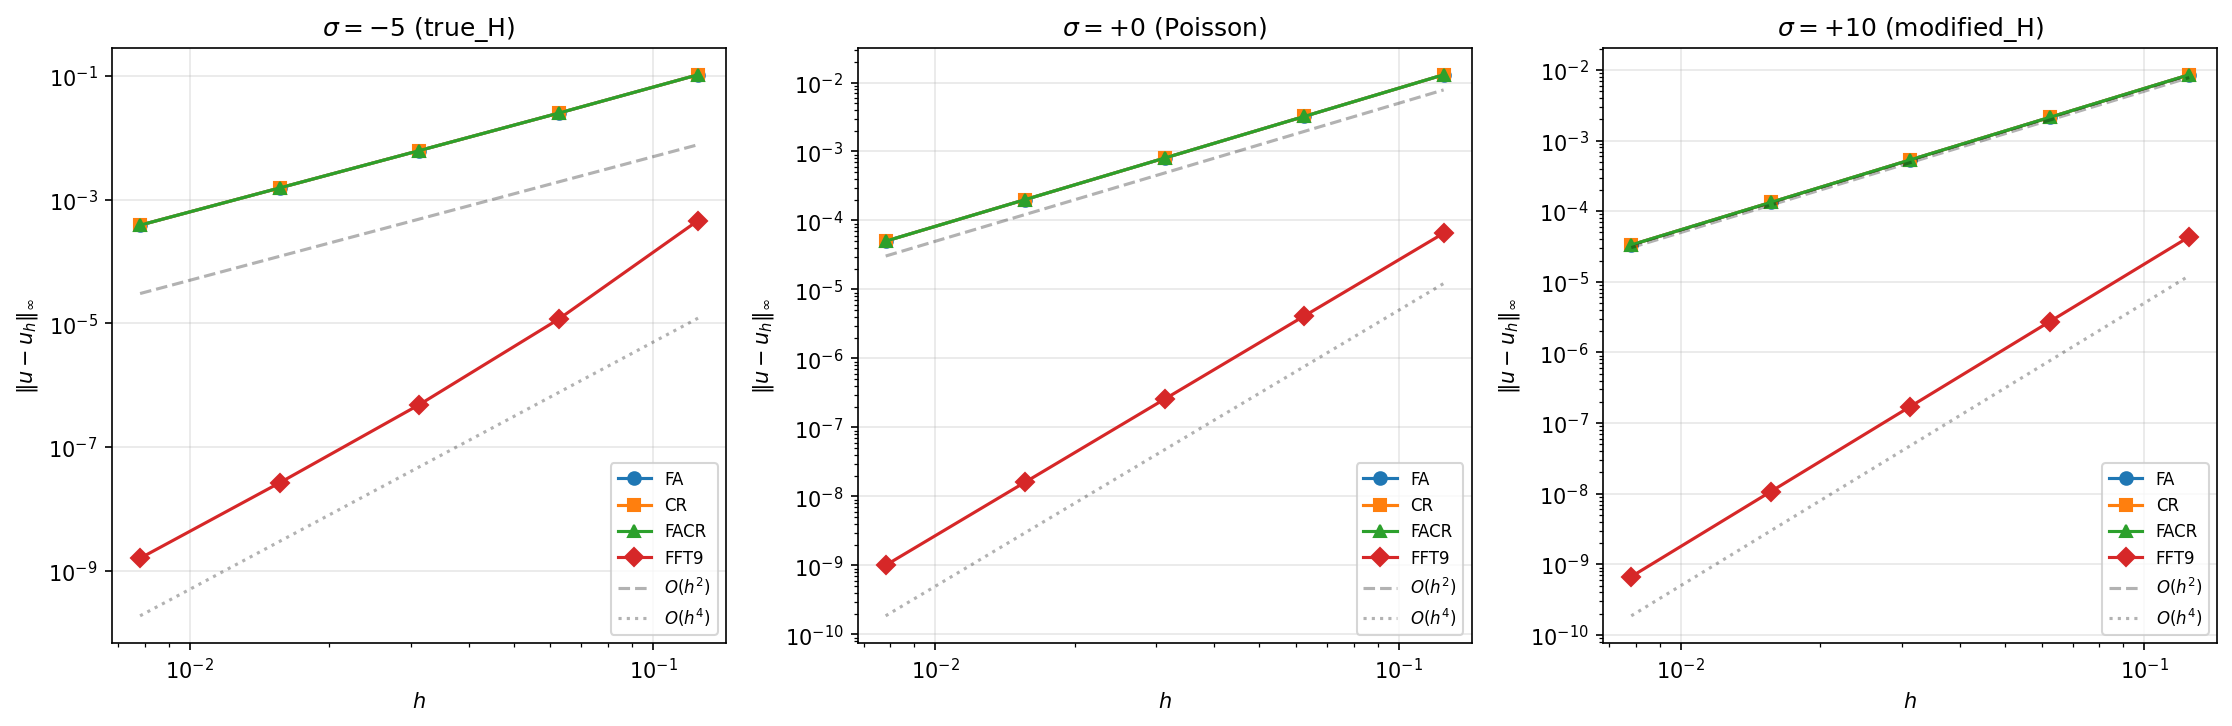
\includegraphics[width=0.82\textwidth]{figures/exp01_convergence.png}
\caption{二阶五点格式与四阶 FFT9 格式的收敛阶验证}
\label{fig:exp01_convergence}
\end{figure}

\begin{table}[htbp]
\centering
\caption{非特征多项式 manufactured solution 的收敛阶（$\sigma=10$）}
\label{tab:exp01_poly_convergence}
\begin{tabular}{cccc}
\toprule
方法 & $n$ & $L_\infty$ 误差 & 观测阶 \\
\midrule
FA / CR / FACR & 33  & $8.92\times10^{-6}$  & $2.00$ \\
FA / CR / FACR & 65  & $2.23\times10^{-6}$  & $2.00$ \\
FA / CR / FACR & 129 & $5.57\times10^{-7}$  & $2.00$ \\
FFT9           & 33  & $8.81\times10^{-9}$  & $4.00$ \\
FFT9           & 65  & $5.51\times10^{-10}$ & $4.00$ \\
FFT9           & 129 & $3.44\times10^{-11}$ & $4.00$ \\
\bottomrule
\end{tabular}
\end{table}

结果表明，FA、CR、FACR 对应的五点差分格式稳定呈现二阶精度，
FFT9 Dirichlet 紧致格式稳定呈现四阶精度。
该结论由 Fourier/Taylor 推导、模态测试和非特征多项式测试共同支撑。
本实验只验证离散格式收敛轨道，不用于判断 GMRES 迭代行为。

\subsection{实验三：非齐次 Dirichlet 边界条件验证}

本实验对应脚本 \texttt{exp02\_nonhom\_bc.py}。
取
\begin{equation}
  u(x,y)=\sin(2\pi x)\sin(3\pi y)+1,
\end{equation}
因此边界上 $g_D=1$，为真正的非齐次 Dirichlet 边界。
对应右端项为
\begin{equation}
  f(x,y)=\bigl((2\pi)^2+(3\pi)^2+\sigma\bigr)\sin(2\pi x)\sin(3\pi y)+\sigma.
\end{equation}
常数 $1$ 的 Laplacian 为零，因此不能写成
$((2\pi)^2+(3\pi)^2+\sigma)u(x,y)$。

\begin{figure}[htbp]
\centering
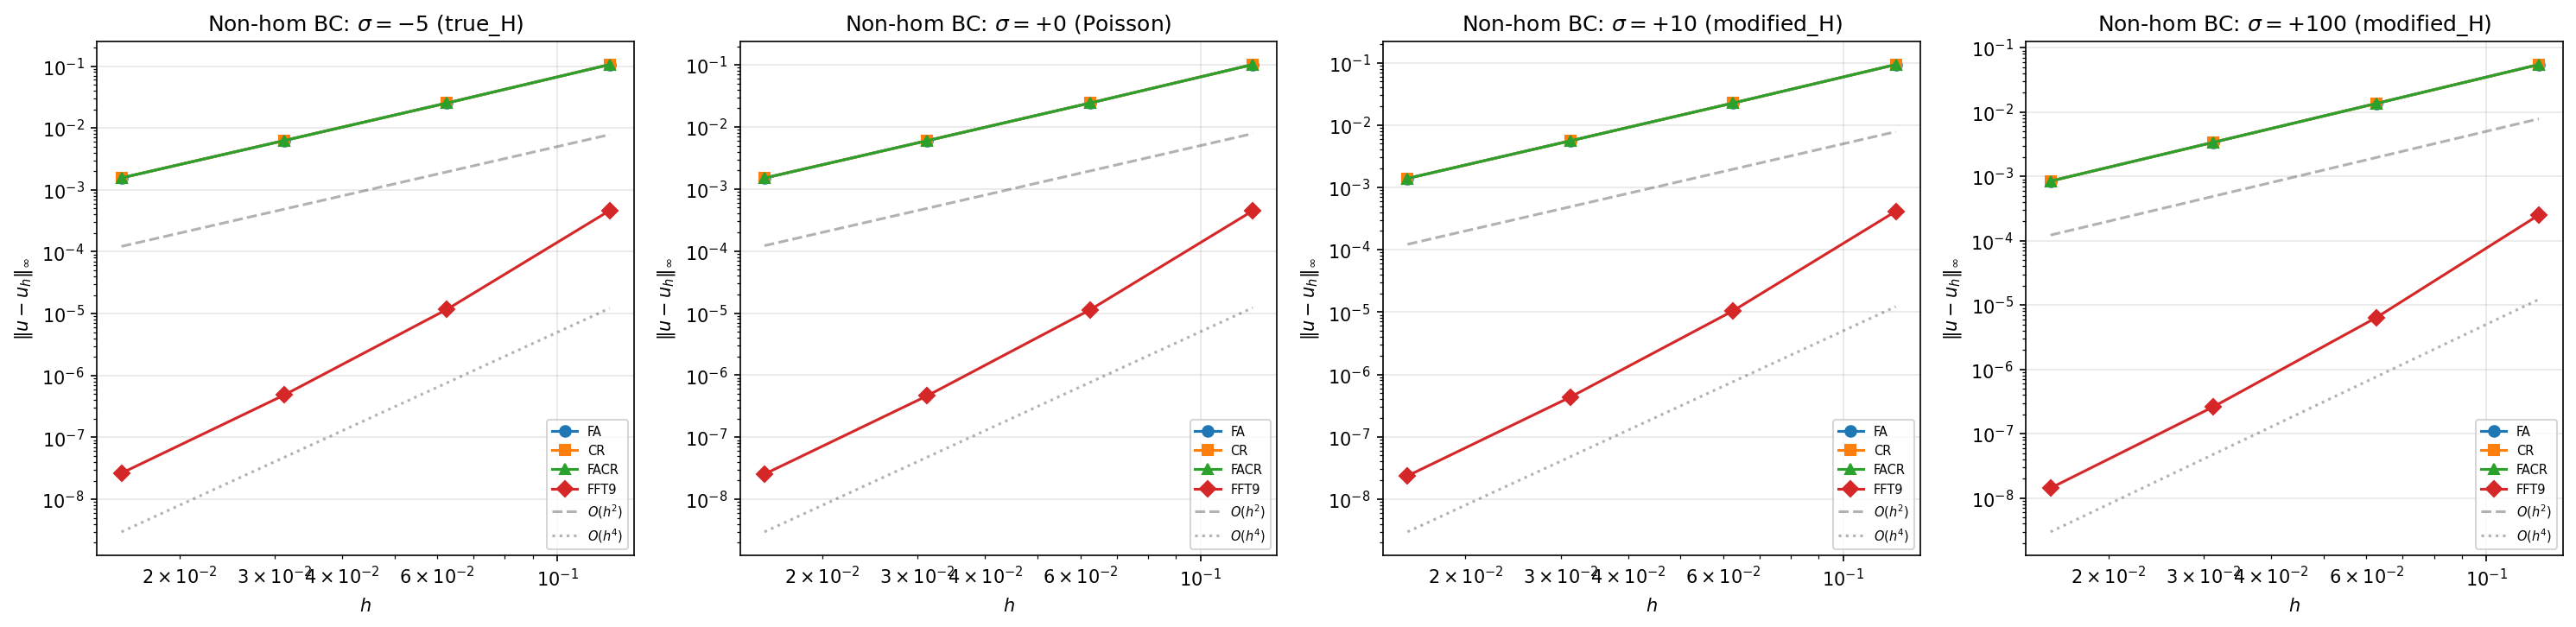
\includegraphics[width=0.82\textwidth]{figures/exp02_nonhom_bc.png}
\caption{非齐次 Dirichlet 边界条件下的误差收敛}
\label{fig:exp02_nonhom_bc}
\end{figure}

\begin{table}[htbp]
\centering
\caption{非齐次 Dirichlet 边界验证（$n=65$）}
\label{tab:exp02_nonhom_bc}
\begin{tabular}{ccccc}
\toprule
$\sigma$ & 方程类型 & 五点格式误差 & 五点格式阶 & FFT9 误差 / 阶 \\
\midrule
$0$    & Poisson     & $1.50\times10^{-3}$ & $2.00$ & $2.54\times10^{-8}$ / $4.19$ \\
$10$   & Modified H. & $1.39\times10^{-3}$ & $2.00$ & $2.36\times10^{-8}$ / $4.19$ \\
$100$  & Modified H. & $8.42\times10^{-4}$ & $2.00$ & $1.43\times10^{-8}$ / $4.19$ \\
$-5$   & True H.     & $1.56\times10^{-3}$ & $2.00$ & $2.64\times10^{-8}$ / $4.19$ \\
\bottomrule
\end{tabular}
\end{table}

表~\ref{tab:exp02_nonhom_bc} 说明，边界值移项符号修正后，
五点格式保持二阶收敛，FFT9 保持约四阶收敛。
这验证了非齐次 Dirichlet 情形下右端项和边界修正的实现一致性，
不涉及 Neumann 或混合边界的九点紧致格式推广。

\subsection{实验四：Neumann 与混合边界条件验证}

本实验对应脚本 \texttt{exp03\_neumann\_mixed.py}。
五点格式通过 ghost-point 方法和对称化 DCT-I/DST-I 组合处理 Neumann 与混合边界。
纯 Neumann Poisson 情形下，误差比较需去除常数偏移；
本文使用与 DCT-I 权重一致的 trapezoid-weighted mean。

\begin{figure}[htbp]
\centering
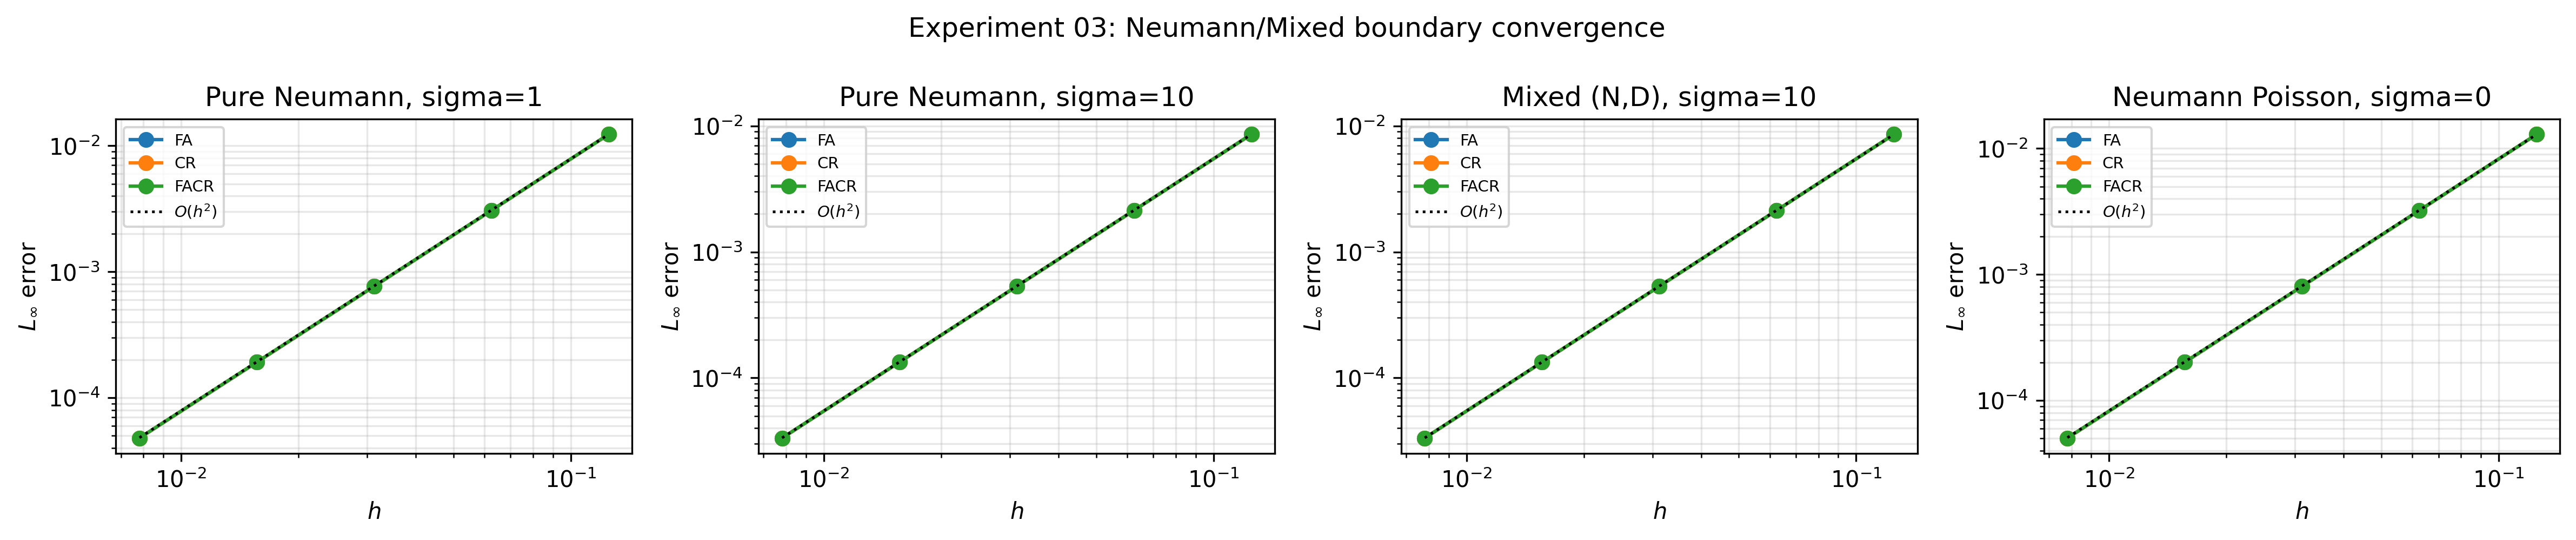
\includegraphics[width=0.82\textwidth]{figures/exp03_neumann_mixed.png}
\caption{Neumann 与混合边界条件下的收敛验证}
\label{fig:exp03_neumann_mixed}
\end{figure}

\begin{table}[htbp]
\centering
\caption{Neumann 与混合边界代表结果（FA，$n=65$）}
\label{tab:exp03_neumann_mixed}
\begin{tabular}{ccccc}
\toprule
子实验 & 边界类型 & $\sigma$ & $L_\infty$ 误差 & 观测阶 \\
\midrule
Pure Neumann & Neumann & $1$  & $1.91\times10^{-4}$ & $2.00$ \\
Pure Neumann & Neumann & $10$ & $1.33\times10^{-4}$ & $2.00$ \\
Mixed        & $(N,D)$ & $10$ & $1.33\times10^{-4}$ & $2.00$ \\
Neumann Poisson & Neumann & $0$ & $2.01\times10^{-4}$ & $2.00$ \\
Mixed        & $(D,N)$ & $10$ & $1.33\times10^{-4}$ & $2.00$ \\
\bottomrule
\end{tabular}
\end{table}

结果表明，ghost-point 对称化方法能够将 Neumann 和混合边界稳定纳入五点 FFT 框架。
需要注意的是，本实验不声称 FFT9 已支持 Neumann 或混合边界四阶格式；
FFT9 的四阶验证仅限 Dirichlet 边界。
因此，实验四验证的是受支持五点求解器的 Neumann/mixed 处理，不证明 FFT9 的 Neumann/mixed 四阶性。

\subsection{实验五：Modified 与 True Helmholtz 的谱指标和 GMRES 行为}

本实验对应脚本 \texttt{exp04\_modified\_vs\_true.py}。
谱指标由五点 Dirichlet 离散分母
\begin{equation}
  d_{p,q}=\lambda_{p,q}+\sigma
\end{equation}
给出。
当 $\sigma>0$ 时，modified Helmholtz 的分母恒正；
当 $\sigma<0$ 时，true Helmholtz 可能因 $-\sigma\approx\lambda_{p,q}$ 出现小分母和病态性。
GMRES 迭代实验使用 Gaussian 型非特征右端项
$f=\exp(-80((x-0.37)^2+(y-0.61)^2))$，
以避免单一 Fourier 模态造成的一步收敛退化。

\begin{figure}[htbp]
\centering
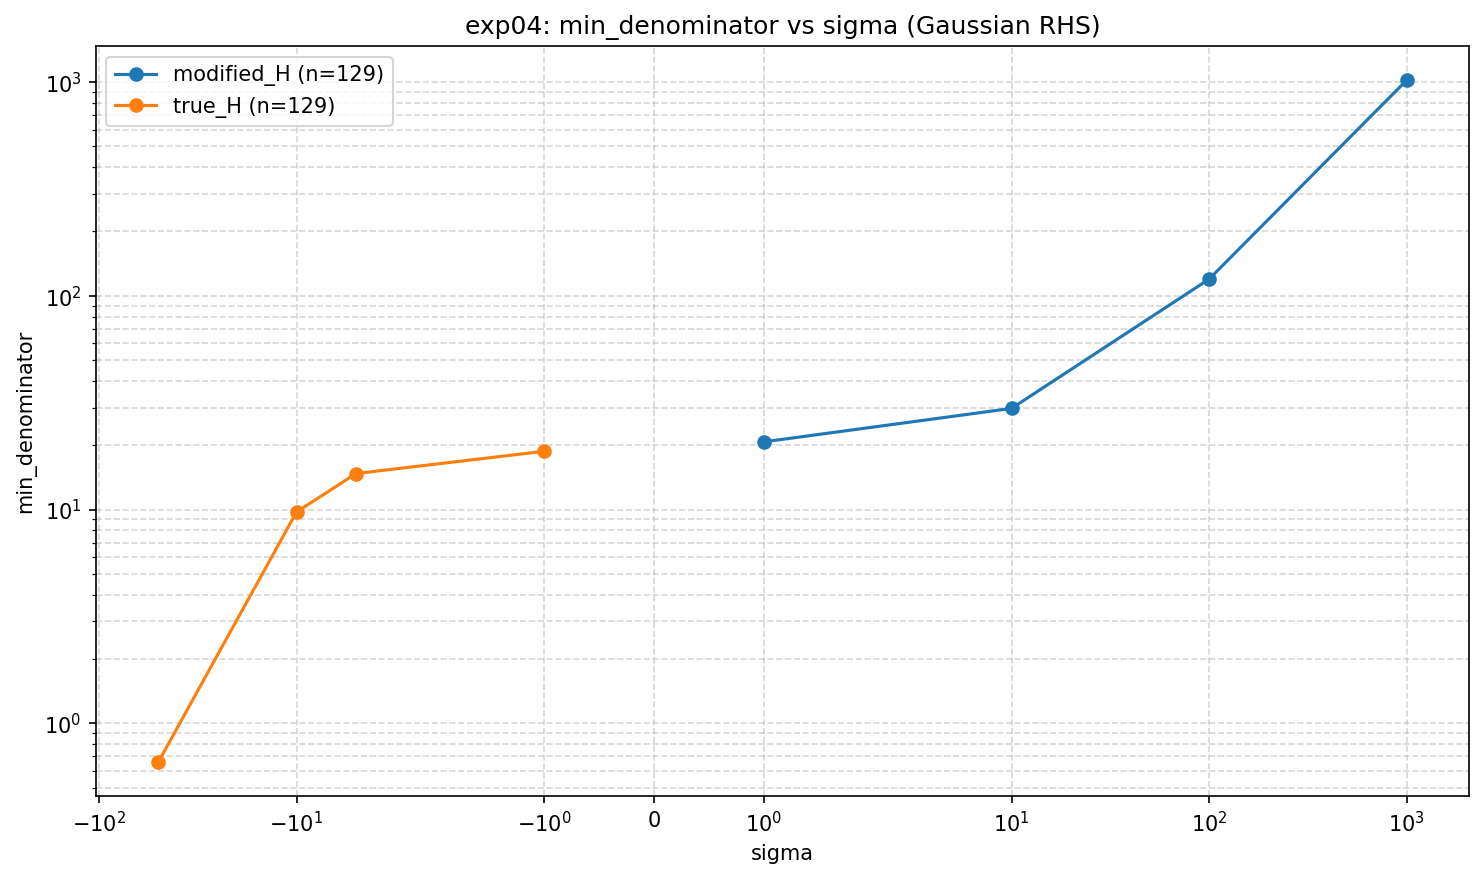
\includegraphics[width=0.48\textwidth]{figures/exp04_min_denom_vs_sigma.png}
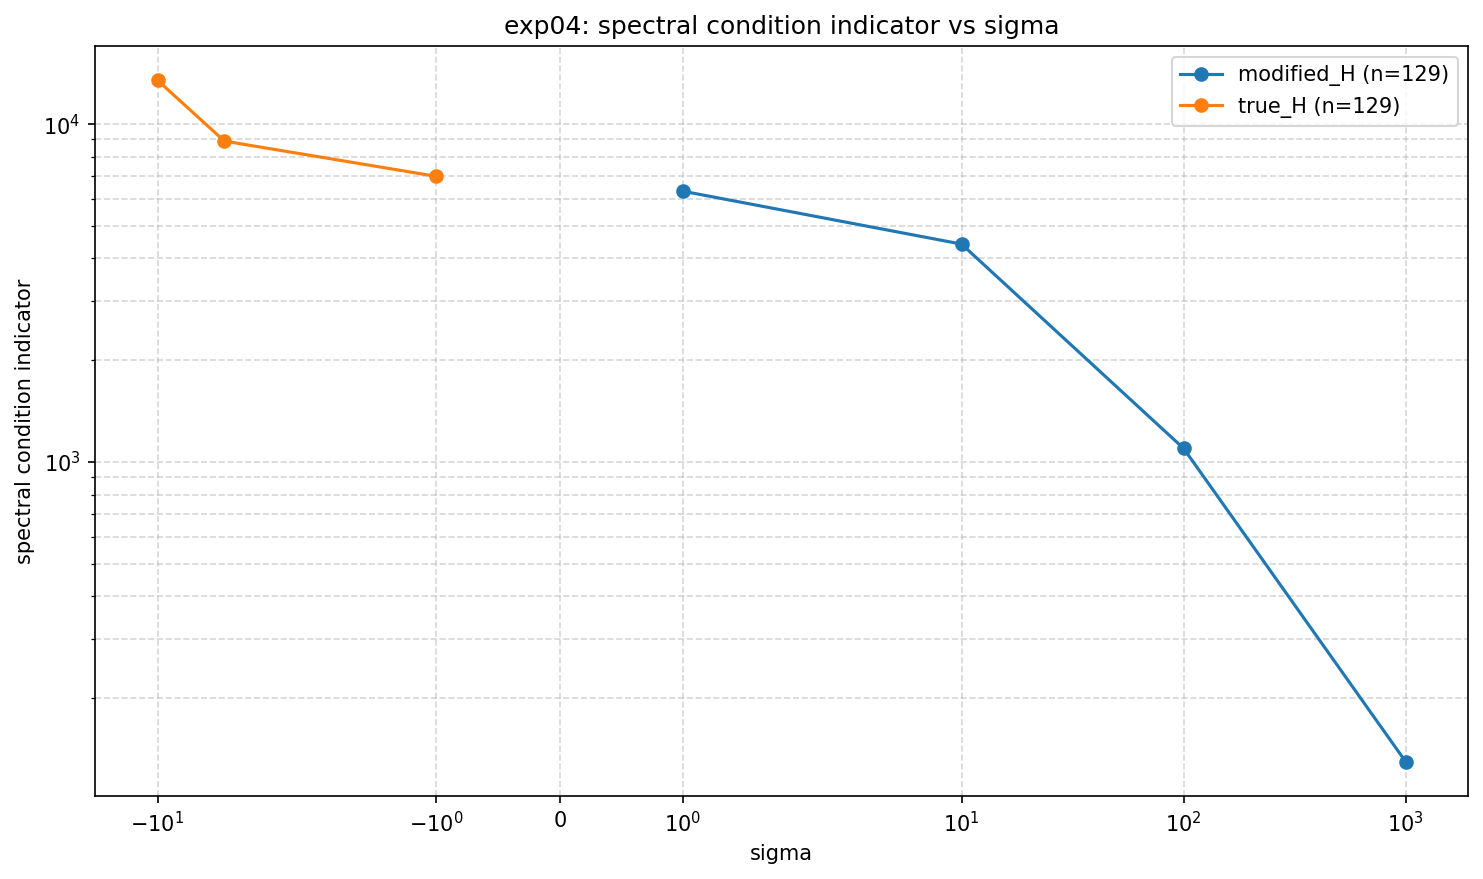
\includegraphics[width=0.48\textwidth]{figures/exp04_spectral_indicator_vs_sigma.png}
\caption{Modified/true Helmholtz 的最小频域分母与谱条件数指标}
\label{fig:exp04_spectral}
\end{figure}

\begin{figure}[htbp]
\centering
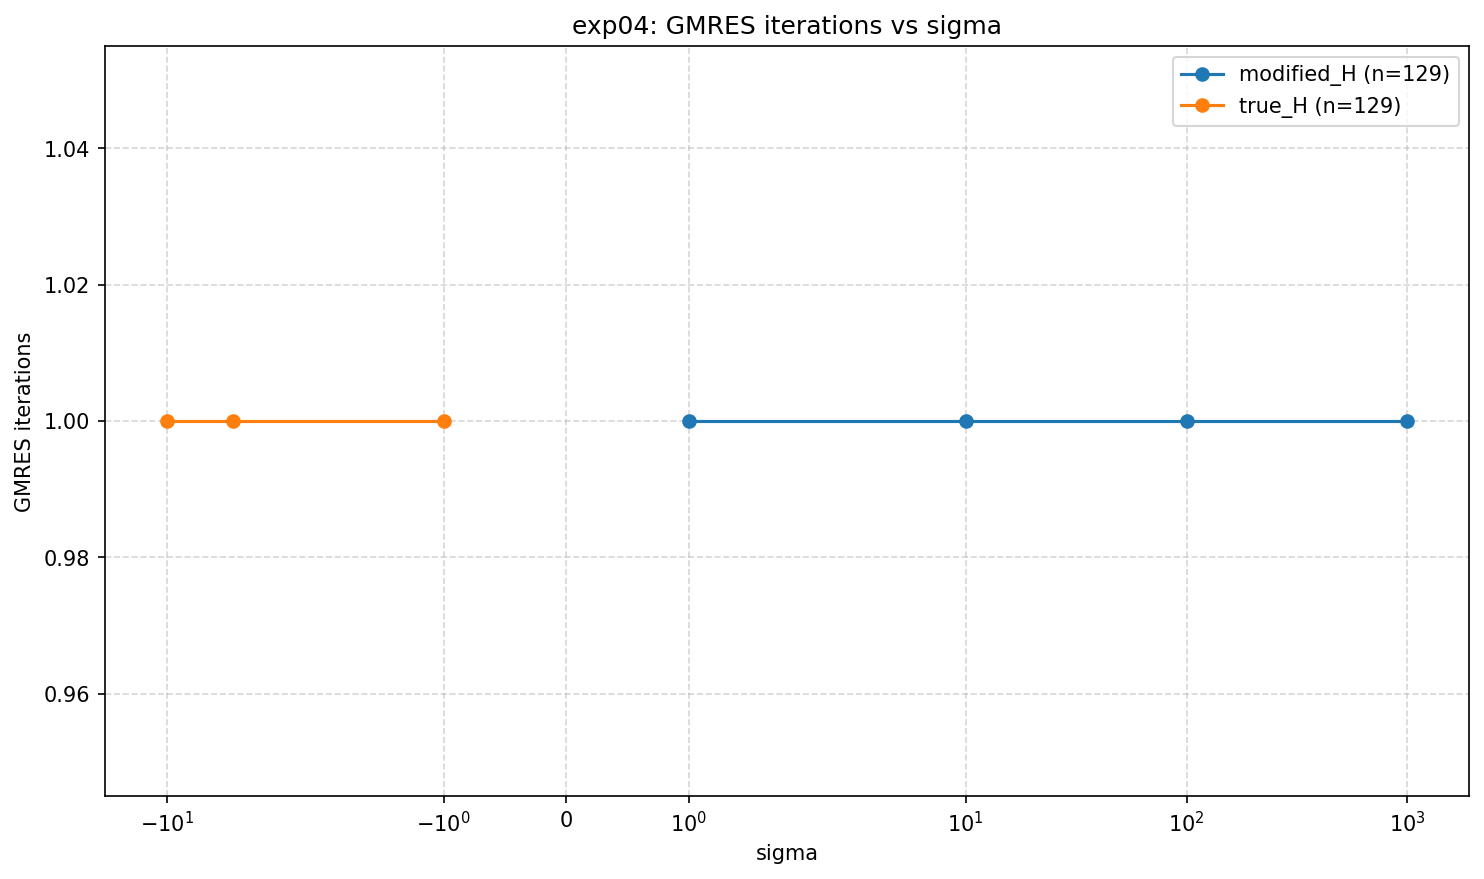
\includegraphics[width=0.68\textwidth]{figures/exp04_gmres_iters_vs_sigma.png}
\caption{Gaussian RHS 下无预处理 GMRES 迭代次数对比}
\label{fig:exp04_gmres}
\end{figure}

\begin{table}[htbp]
\centering
\caption{Modified/true Helmholtz 谱指标与 GMRES 迭代次数（$n=33$）}
\label{tab:exp04_mod_true}
\begin{tabular}{cccccc}
\toprule
$\sigma$ & 方程类型 & $d_{\min}$ & 谱指标 & GMRES 迭代 & 状态 \\
\midrule
$1$    & Modified & $20.72$ & $3.94\times10^2$ & $256$ & 收敛 \\
$10$   & Modified & $29.72$ & $2.75\times10^2$ & $203$ & 收敛 \\
$100$  & Modified & $119.72$ & $6.91\times10^1$ & $91$ & 收敛 \\
$1000$ & Modified & $1019.72$ & $8.99$ & $27$ & 收敛 \\
\midrule
$-1$   & True & $18.72$ & $4.36\times10^2$ & $270$ & 收敛 \\
$-5$   & True & $14.72$ & $5.55\times10^2$ & $319$ & 收敛 \\
$-10$  & True & $9.72$  & $8.39\times10^2$ & $428$ & 收敛 \\
$-50$  & True & $0.79$  & $1.03\times10^4$ & $>500$ & 近共振 \\
\bottomrule
\end{tabular}
\end{table}

表~\ref{tab:exp04_mod_true} 显示，modified Helmholtz 随 $\sigma$ 增大远离小分母，
谱指标改善，无预处理 GMRES 迭代次数下降；
true Helmholtz 随 $|\sigma|$ 接近离散 Laplacian 特征值而出现小分母风险，
GMRES 迭代变慢甚至在给定上限内未收敛。
该实验只观察 Gaussian RHS 下无预处理 GMRES 的参数敏感性，不构成完整迭代法性能研究。

\subsection{实验六：True Helmholtz 近共振扫描}

本实验对应脚本 \texttt{exp05\_true\_helmholtz\_resonance.py}。
取 $n=65$，目标模态 $(p,q)=(2,1)$，
离散特征值 $\lambda_{2,1}^h\approx49.3143$，
令
\begin{equation}
  \sigma=-(\lambda_{2,1}^h+\delta),
\end{equation}
并扫描正负两侧的小扰动 $\delta$。
右端项仍采用 Gaussian 型非特征函数。

\begin{figure}[htbp]
\centering
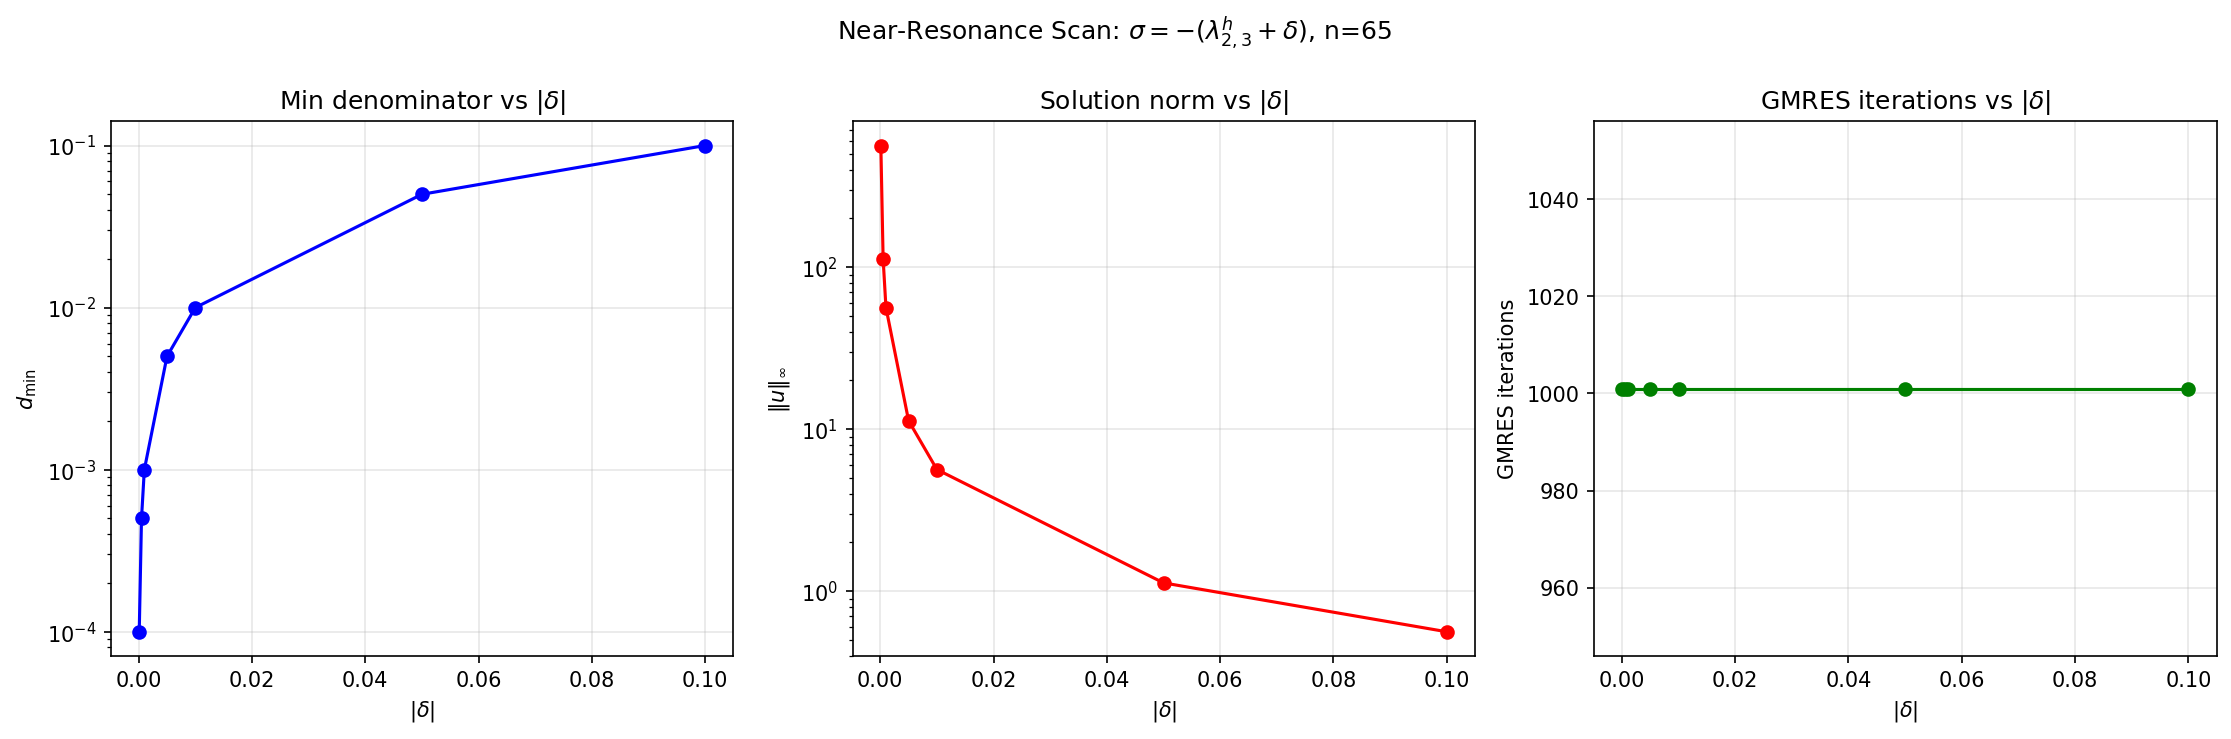
\includegraphics[width=\textwidth]{figures/exp05_resonance.png}
\caption{True Helmholtz 近共振扫描：$d_{\min}$、解范数和 GMRES 迭代随 $|\delta|$ 的变化}
\label{fig:exp05_resonance}
\end{figure}

\begin{table}[htbp]
\centering
\caption{近共振扫描代表数据（$n=65$）}
\label{tab:exp05_resonance}
\begin{tabular}{cccc}
\toprule
$|\delta|$ & $d_{\min}$ & $\|u\|_\infty$ & GMRES 迭代 \\
\midrule
$10^{-1}$ & $1.00\times10^{-1}$ & $1.32$ & $1001$（未收敛） \\
$10^{-2}$ & $1.00\times10^{-2}$ & $13.19$ & $1001$（未收敛） \\
$10^{-3}$ & $1.00\times10^{-3}$ & $131.92$ & $1001$（未收敛） \\
$10^{-4}$ & $1.00\times10^{-4}$ & $1.32\times10^{3}$ & $1001$（未收敛） \\
\bottomrule
\end{tabular}
\end{table}

结果验证了第\ref{sec:helmholtz}章的频域分析：
当 $\kappa^2$ 接近离散 Laplacian 特征值时，最小分母 $d_{\min}$ 下降，
对应模态的解分量被放大，线性系统变得病态。
无预处理 GMRES 在这些近共振参数下无法在给定迭代上限内收敛，
说明 true Helmholtz 问题通常需要 shifted-Laplacian 等预处理技术。
该结论仅针对 true Helmholtz 近共振扫描，不外推为一般波数性能比较。

\subsection{实验总结}

本章将原有大量历史实验压缩为六组可复现的核心实验。
实验一验证 FFT 类五点求解器与稀疏直接解的一致性；
实验二验证五点格式二阶和 FFT9 Dirichlet 紧致格式四阶；
实验三验证非齐次 Dirichlet 右端项与边界修正符号；
实验四验证 Neumann 与混合边界在五点 FFT 框架中的处理；
实验五和实验六分别从远离共振的谱指标和近共振扫描两方面说明 modified/true Helmholtz 的本质差异。

由这些实验可得：
\begin{itemize}[itemsep=2pt]
  \item 对规则单位正方形和均匀网格，FFT 直接法能够高精度求解对应离散系统；
  \item 五点格式和 FFT9 Dirichlet 紧致格式分别呈现二阶和四阶精度；
  \item 非齐次 Dirichlet、Neumann 与混合边界的实现已通过离散一致性或收敛阶验证；
  \item modified Helmholtz 与 true Helmholtz 的差异来自频域分母结构，不能把二者的迭代行为混写；
  \item true Helmholtz 在近共振时出现解范数放大和无预处理 GMRES 收敛困难。
\end{itemize}

本章不再保留无统计重复计时、装饰性热力图、GMRES 重启参数图或单独复杂度趋势图作为核心证据。
这些材料可作为探索性输出留存在图像目录中，但不参与本文最终结论。
